%!!!!!!!!!!!!!!!!!!!!!!!!!!!!!!!!!!!!!!!!!!!!!!!!!!!!!!!!!!!!!!!!!!!!!!!!!!!!!!!
%
%               Auto Generated by tikzpy. Try not to modify the TeX comments
%               of the form "%__begin__@TikzPy__#id__==__(...)".
%
%!!!!!!!!!!!!!!!!!!!!!!!!!!!!!!!!!!!!!!!!!!!!!!!!!!!!!!!!!!!!!!!!!!!!!!!!!!!!!!!

%__begin__@TikzPy__#id__==__(0)
\begin{center}
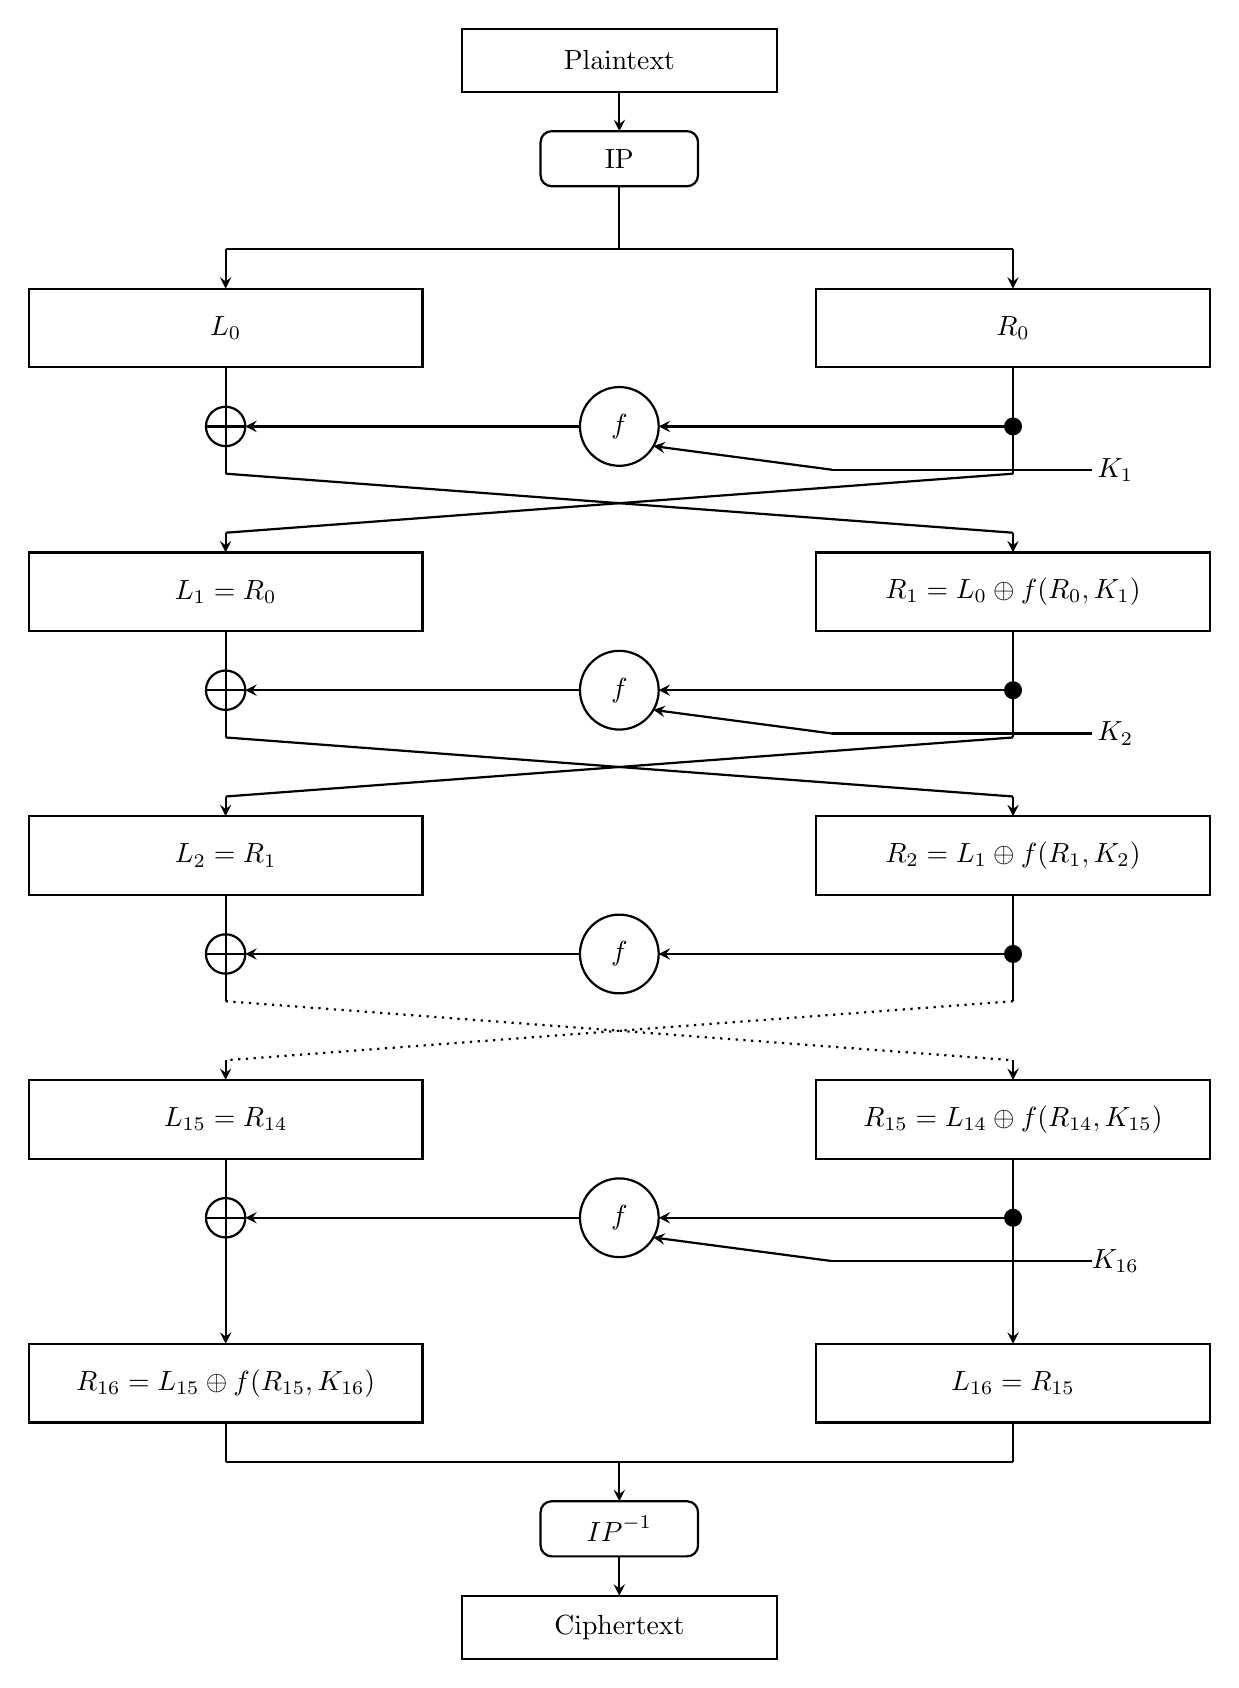
\begin{tikzpicture}[>=stealth, thick]
    \draw (0, 0) rectangle (4, 0.8);
    \node at (2.0, 0.4) { Plaintext };
    \draw[->] (2.0, 0) to (2.0, -0.5);
    \draw[rounded corners] (1.0, -1.2) rectangle (3.0, -0.5);
    \node at (2.0, -0.85) { IP };
    \draw (2.0, -1.2) to (2.0, -2.0);
    \draw (2.0, -2.0) to (-3.0, -2.0);
    \draw (2.0, -2.0) to (7.0, -2.0);
    \draw[->] (-3.0, -2.0) to (-3.0, -2.5);
    \draw[->] (7.0, -2.0) to (7.0, -2.5);
    \draw (-5.5, -3.5) rectangle (-0.5, -2.5);
    \node at (-3.0, -3.0) { $L_0$ };
    \draw (4.5, -3.5) rectangle (9.5, -2.5);
    \node at (7.0, -3.0) { $R_0$ };
    \draw (-3.0, -3.5) to (-3.0, -4.0);
    \draw (-3.0, -4.25) circle (0.25cm);
    \draw (-3.0, -4.0) to (-3.0, -4.5);
    \draw (-3.25, -4.25) to (-2.75, -4.25);
    \draw (7.0, -3.5) to (7.0, -4.25);
    \draw[fill] (7.0, -4.25) circle (0.1cm);
    \draw (2.0, -4.25) circle (0.5cm);
    \node at (2.0, -4.25) { $f$ };
    \draw[->] (6.9, -4.25) to (2.5, -4.25);
    \draw[->] (1.5, -4.25) to (-2.75, -4.25);
    \draw (-3.0, -4.5) to (-3.0, -4.85);
    \draw (-3.0, -4.85) to (7.0, -5.6);
    \draw[->] (7.0, -5.6) to (7.0, -5.85);
    \draw (7.0, -4.35) to (7.0, -4.85);
    \draw (7.0, -4.85) to (-3.0, -5.6);
    \draw[->] (-3.0, -5.6) to (-3.0, -5.85);
    \draw (8.0, -4.8) to (4.7, -4.8);
    \draw[->] (4.7, -4.8) to (2.433012701892219, -4.5);
    \node at (8.3, -4.8) { $K_1$ };
    \draw (-5.5, -6.85) rectangle (-0.5, -5.85);
    \node at (-3.0, -6.35) { $L_1=R_0$ };
    \draw (4.5, -6.85) rectangle (9.5, -5.85);
    \node at (7.0, -6.35) { $R_1 = L_0 \oplus f(R_0, K_1)$ };
    \draw (-3.0, -6.85) to (-3.0, -7.35);
    \draw (-3.0, -7.6) circle (0.25cm);
    \draw (-3.0, -7.35) to (-3.0, -7.85);
    \draw (-3.25, -7.6) to (-2.75, -7.6);
    \draw (7.0, -6.85) to (7.0, -7.6);
    \draw[fill] (7.0, -7.6) circle (0.1cm);
    \draw (2.0, -7.6) circle (0.5cm);
    \node at (2.0, -7.6) { $f$ };
    \draw[->] (6.9, -7.6) to (2.5, -7.6);
    \draw[->] (1.5, -7.6) to (-2.75, -7.6);
    \draw (-3.0, -7.85) to (-3.0, -8.2);
    \draw (-3.0, -8.2) to (7.0, -8.95);
    \draw[->] (7.0, -8.95) to (7.0, -9.2);
    \draw (7.0, -7.699999999999999) to (7.0, -8.2);
    \draw (7.0, -8.2) to (-3.0, -8.95);
    \draw[->] (-3.0, -8.95) to (-3.0, -9.2);
    \draw (8.0, -8.149999999999999) to (4.7, -8.149999999999999);
    \draw[->] (4.7, -8.149999999999999) to (2.433012701892219, -7.85);
    \node at (8.3, -8.149999999999999) { $K_2$ };
    \draw (-5.5, -10.2) rectangle (-0.5, -9.2);
    \node at (-3.0, -9.7) { $L_2=R_1$ };
    \draw (4.5, -10.2) rectangle (9.5, -9.2);
    \node at (7.0, -9.7) { $R_2 = L_1 \oplus f(R_1, K_2)$ };
    \draw (-3.0, -10.2) to (-3.0, -10.7);
    \draw (-3.0, -10.95) circle (0.25cm);
    \draw (-3.0, -10.7) to (-3.0, -11.2);
    \draw (-3.25, -10.95) to (-2.75, -10.95);
    \draw (7.0, -10.2) to (7.0, -10.95);
    \draw[fill] (7.0, -10.95) circle (0.1cm);
    \draw (2.0, -10.95) circle (0.5cm);
    \node at (2.0, -10.95) { $f$ };
    \draw[->] (6.9, -10.95) to (2.5, -10.95);
    \draw[->] (1.5, -10.95) to (-2.75, -10.95);
    \draw (-3.0, -11.2) to (-3.0, -11.549999999999999);
    \draw[dotted] (-3.0, -11.549999999999999) to (7.0, -12.299999999999999);
    \draw[->] (7.0, -12.299999999999999) to (7.0, -12.549999999999999);
    \draw (7.0, -11.049999999999999) to (7.0, -11.549999999999999);
    \draw[dotted] (7.0, -11.549999999999999) to (-3.0, -12.299999999999999);
    \draw[->] (-3.0, -12.299999999999999) to (-3.0, -12.549999999999999);
    \draw (-5.5, -13.549999999999999) rectangle (-0.5, -12.549999999999999);
    \node at (-3.0, -13.049999999999999) { $L_{15}=R_{14}$ };
    \draw (4.5, -13.549999999999999) rectangle (9.5, -12.549999999999999);
    \node at (7.0, -13.049999999999999) { $R_{15} = L_{14} \oplus f(R_{14}, K_{15})$ };
    \draw (-3.0, -13.549999999999999) to (-3.0, -14.049999999999999);
    \draw (-3.0, -14.299999999999999) circle (0.25cm);
    \draw (-3.0, -14.049999999999999) to (-3.0, -14.549999999999999);
    \draw (-3.25, -14.299999999999999) to (-2.75, -14.299999999999999);
    \draw (7.0, -13.549999999999999) to (7.0, -14.299999999999999);
    \draw[fill] (7.0, -14.299999999999999) circle (0.1cm);
    \draw (2.0, -14.299999999999999) circle (0.5cm);
    \node at (2.0, -14.299999999999999) { $f$ };
    \draw[->] (6.9, -14.299999999999999) to (2.5, -14.299999999999999);
    \draw[->] (1.5, -14.299999999999999) to (-2.75, -14.299999999999999);
    \draw (-3.0, -14.549999999999999) to (-3.0, -14.899999999999999);
    \draw (-3.0, -14.899999999999999) to (-3.0, -15.649999999999999);
    \draw[->] (7.0, -15.649999999999999) to (7.0, -15.899999999999999);
    \draw (7.0, -14.399999999999999) to (7.0, -14.899999999999999);
    \draw (7.0, -14.899999999999999) to (7.0, -15.649999999999999);
    \draw[->] (-3.0, -15.649999999999999) to (-3.0, -15.899999999999999);
    \draw (8.0, -14.849999999999998) to (4.7, -14.849999999999998);
    \draw[->] (4.7, -14.849999999999998) to (2.433012701892219, -14.549999999999999);
    \node at (8.3, -14.849999999999998) { $K_{16}$ };
    \draw (-5.5, -16.9) rectangle (-0.5, -15.899999999999999);
    \node at (-3.0, -16.4) { $R_{16} = L_{15}\oplus f(R_{15}, K_{16})$ };
    \draw (4.5, -16.9) rectangle (9.5, -15.899999999999999);
    \node at (7.0, -16.4) { $L_{16} = R_{15}$ };
    \draw (-3.0, -16.9) to (-3.0, -17.4);
    \draw (7.0, -16.9) to (7.0, -17.4);
    \draw (-3.0, -17.4) to (2.0, -17.4);
    \draw (7.0, -17.4) to (2.0, -17.4);
    \draw[->] (2.0, -17.4) to (2.0, -17.9);
    \draw[rounded corners] (1.0, -18.599999999999998) rectangle (3.0, -17.9);
    \node at (2.0, -18.25) { $\text{IP}^{-1}$ };
    \draw[->] (2.0, -18.599999999999998) to (2.0, -19.099999999999998);
    \draw (0.0, -19.9) rectangle (4.0, -19.099999999999998);
    \node at (2.0, -19.5) { Ciphertext };
\end{tikzpicture}
\end{center}
%__end__@TikzPy__#id__==__(0)
